\documentclass{beamer}
\usetheme{Madrid}

\usepackage{amsmath, amssymb, amsthm}
\usepackage{graphicx}
\usepackage{listings}
\usepackage{gensymb}
\usepackage{minted}
\usemintedstyle{friendly}
\definecolor{bg}{rgb}{0.95,0.95,0.95}
\usepackage[utf8]{inputenc}
\usepackage{hyperref}
\usepackage{gvv}\begin{document}
\title{10.3.2.4.1}
\author{EE24BTECH11012 \\ BHAVANISANKAR G S }
\date{\today}
\frame{\titlepage}

\begin{frame}
\frametitle{Question}
Determine if the system of equations
\begin{align}
	x + y &= 5 \label{eq:qn} \\
	2x + 2y &= 10
\end{align}
is consistent or not. If consistent, obtain the solution graphically.
\end{frame}

\begin{frame}
\frametitle{Solution Outline}
\begin{enumerate}
\item Formulate the given system of equations in matrix form.
\item Factorize the matrix as
\begin{align}
	\vec{A} &= \vec{L} \vec{U} \\
	\vec{L} &= Lower triangular \\
	\vec{U} &= Upper triangular
\end{align}
\item Solve the equation
\begin{align}
	\vec{L} \vec{U} \vec{x} &= \vec{B} \\
	\implies \vec{L} \vec{y} &= \vec{B} \label{eq:lu1} \\
	\vec{U} \vec{x} &= \vec{y} \label{eq:lu2}
\end{align}
\end{enumerate}
\end{frame}

\begin{frame}
\frametitle{Algorithm}
Let $\vec{A}$ be an $n \times n$ matrix. Initialize $\vec{L}$ to an $n \times n$ Identity matrix. Initialize $\vec{U}$ to a zero matrix.
	\begin{align}
		L &= \myvec{1 & 0 & \cdots & 0 \\
		            0 & 1 & \cdots & 0 \\
		            \vdots & \vdots & \ddots & \vdots \\
		            0 & 0 & \cdots & 1} \\
		U &= \myvec{0 & 0 & \cdots & 0 \\
			    0 & 0 & \cdots & 0 \\
                            \vdots & \vdots & \ddots & \vdots \\
                            0 & 0 & \cdots & 0}
	\end{align}
\end{frame}

\begin{frame}
	\item For each row $i$ from $0$ to $n-1$ :
	\begin{enumerate}
		\item For each column $j$ from $i$ to $n-1$ : 
		\begin{align}
			U_{ij} &= A_{ij} - \sum_{k=0}^{i-1} L_{ik} U_{kj}
		\end{align}
		\item For each row $j$ from $i+1$ to $n-1$ :
		\begin{align}
			L_{ji} &= \frac{1}{U_{ii}} \brak{A_{ij} - \sum_{k=0}^{i-1} L_{jk} U_{ki}}
		\end{align}
	\end{enumerate}
	\item Repeat the above step for all $i = 0,1,\dots,n-1$
	\item After all the iterations
	\begin{align}
		\vec{A} &= \vec{L} \vec{U}
	\end{align}
\end{frame}

\begin{frame}
\frametitle{Solution}
For the given question, 
\begin{align}
	\vec{A} &= \myvec{1 & 1 \\ 2 & 2} \\
	\vec{L} &= \myvec{1 & 0 \\ 2 & 1} \\
	\vec{U} &= \myvec{1 & 1 \\ 0 & 0}
\end{align}
Using \eqref{eq:lu1}, we have
\begin{align}
	\myvec{1 & 0 \\ 2 & 1} \myvec{y_{1} \\ y_{2}} &= \myvec{5 \\ 10}
\end{align}
By the method of \textbf{Forward substitution}, we have
\begin{align}
	\myvec{y_{1} \\ y_{2}} &= \myvec{5 \\ 0}
\end{align}

\end{frame}

\begin{frame}
Similarly, 
\begin{align}
	\myvec{1 & 1 \\ 0 & 0} \myvec{x_{1} \\ x_{2}} &= \myvec{5 \\ 0} \label{eq:ans2}
\end{align}
It can be seen that
\begin{align}
	x_{1} + x_{2} &= 5 \label{eq:ans} \\
	0 &= 0
\end{align}
which is the same as the equation given in question, indicating that the given system of equations has infinite number of solutions, and hence, the system is consistent.
\end{frame}

\begin{frame}
\frametitle{Cramer's Rule}
This question can also be solved by \textbf{Cramer's Rule}. According to this rule, the solution of the equation
\begin{align}
	\vec{A} \vec{x} &= \vec{b} \label{eq:solve}
\end{align}
is given by
\begin{align}
	\vec{x_{i}} &= \frac{D_{i}}{|A|}
\end{align}
where, $D_{i}$ is the discriminant of the matrix in which the $i^{th}$ column of $\vec{D}$ replaced by the vector $\vec{b}$. \\
If $|A| = 0$, then ( in case of a $2 \times 2$ matrix )
\begin{enumerate}
	\item If $D_{1} = 0 \text{ and } D_{2} = 0$, then the system has infinitely many solutions. 
	\item If $D_{i} \neq 0 \text{ for some } i < 2$, then the system has no solution.
\end{enumerate}
\end{frame}

\begin{frame}
\frametitle{Solution - Cramer's Rule}

For the given question, 
\begin{align}
	\vec{A} &= \myvec{1 & 1 \\ 2 & 2} \\
	\implies |A| &= 0 \\
	\vec{D_{1}} &= \myvec{1 & 5 \\ 2 & 10} \\
	\implies |D_{1}| &= 0 \\
	\vec{D_{2}} &= \myvec{1 & 5 \\ 2 & 10} \\
	\implies |D_{1}| &= 0 
\end{align}
Hence, the system has infinitely many solutions, and is consistent.
\end{frame}

\begin{frame}
\frametitle{QR method}
Consider
\begin{align}
	\vec{A} &= \vec{Q} \vec{R} \\
	\vec{Q} &- Orthonormal \\
	\vec{R} &- Upper triangular
\end{align}
The equation \eqref{eq:solve} can be simplified to
\begin{align}
	\vec{Q} \vec{R} \vec{x} &= \vec{B} \\
	\vec{R} \vec{x} &= \vec{Q}^{T} \vec{B}
\end{align}
This can then be solved using \textbf{Back substitution}.
\end{frame}

\begin{frame}
\frametitle{Solution - QR method}
Using the \textbf{Gram-Schmidt orthogonalisation}, we have
\begin{align}
	\vec{A} &= \myvec{1 & 1 \\ 2 & 2} \\
		&= \myvec{\frac{1}{\sqrt{5}} & 0 \\ \frac{2}{\sqrt{5}} & 0} \myvec{\sqrt{5} & \sqrt{5} \\ 0 & 0} \\
	\implies \myvec{\sqrt{5} & \sqrt{5} \\ 0 & 0} \myvec{x \\ y} &= \myvec{\frac{1}{\sqrt{5}} & \frac{2}{\sqrt{5}} \\ 0 & 0} \myvec{5 \\ 10}
\end{align}
which again simplifies to \eqref{eq:ans2} indicating that the given system is consistent with infinite number of solutions.
\end{frame}

\begin{frame}
\frametitle{Plot}
\begin{figure}[h]
\centering
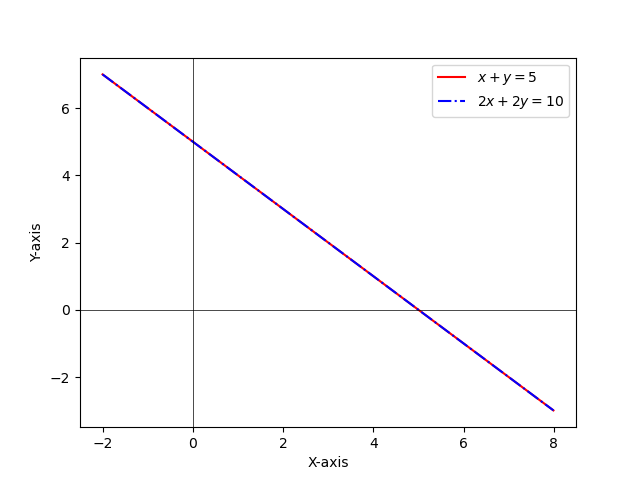
\includegraphics[width=\columnwidth]{figs/fig.png}
\caption{System of consistent equations with infinitely many solutions}
\label{fig:Plot1} 
\end{figure}
\end{frame}
\end{document}
